%\documentclass[preprint]{aastex}  % USE THIS TO MAKE BIB, THEN FORMAT USING EMULATEAPJ
\documentclass[twocolumn,numberedappendix]{emulateapj}
\shorttitle{PSA64}
\shortauthors{Ali, et al.}

\usepackage{amsmath}
\usepackage{graphicx}
\usepackage[figuresright]{rotating}
%\usepackage{rotating}
\usepackage{natbib}
%\usepackage{pdflscape}
%\usepackage{lscape}
\citestyle{aa}

\def\b{\mathbf{b}}
\def\k{\mathbf{k}}
\def\r{\mathbf{r}}
\def\q{\mathbf{q}}
\def\b{\mathbf{b}}
\def\kp{\mathbf{k}^\prime}
\def\kpp{\mathbf{k}^{\prime\prime}}
\def\V{\mathbb{V}}
\def\expval#1{\langle #1 \rangle}
\def\At{\tilde{A}}
\def\Vt{\tilde{V}}
\def\Tt{\tilde{T}}
\def\tb{\langle T_b\rangle}
\newcommand{\vis}{\mathbf{v}}
\newcommand{\x}{\mathbf{x}}
\newcommand{\xhat}{\hat{\mathbf{x}}}
\newcommand{\A}{\mathbf{A}}
\newcommand{\N}{\mathbf{N}}
\newcommand{\rhat}{\hat{\mathbf{r}}}

\begin{document}
\title{PSA-64 Power Spectrum}

\author{
Zaki S. Ali\altaffilmark{1},
Aaron R. Parsons\altaffilmark{1,2},
Jeff Zheng,
Jonathan C. Pober\altaffilmark{4},
James E. Aguirre\altaffilmark{3},
David R. DeBoer\altaffilmark{2},
Daniel C. Jacobs\altaffilmark{8},
Adrian Liu\altaffilmark{1},
David F. Moore\altaffilmark{3}
% XXX if includes paper data, needs full author list
}
%\tableofcontents

\altaffiltext{1}{Astronomy Dept., U. California, Berkeley, CA}
\altaffiltext{2}{Radio Astronomy Lab., U. California, Berkeley, CA}
\altaffiltext{3}{Dept. of Physics and Astronomy, U. Pennsylvania, Philadelphia, PA}
\altaffiltext{4}{Physics Dept.  U. Washington, Seattle, WA}
\altaffiltext{8}{School of Earth and Space Exploration, Arizona State U., Tempe, AZ}

\begin{abstract}
\end{abstract}

% XXX fringe weighting profile
% XXX delay spectrum not violated by freq-dependent fringe rate weights

\section{Introduction}
The Donald C. Backer Precision Array for Probing the Epoch of Reionization
(PAPER) is a dedicated experiment to measure the power spectrum of highly
redshifted 21 cm emission during the Epoch of Reionization. PAPER is but one
experiment that aims to detect this faint signal. Other telescopes that have the
same goal are the Giant Meter-wave Radio Telescope (GMRT), the LOw Frequency
ARray (LOFAR), and the Murchison Widefield Array (MWA). PAPER currently consists
of 128 dual-polarization antennaes in a 100-200MHz band out in the Karoo desert
in South Africa. 

The current best upper limit on 21 cm signal level is at $(41 mK)^{2}$ at
$k=.27 h \text{Mpc}^{-1}$ which was measured by PAPER in a 32 antenna redundant
configuration (\ref{parsons_et_al2014a}). This limit was acheived by using the
delay-spectrum technique to remove foregrounds and using the  maximum
redundancy array to repeatedly measure the same fourier mode, boosting
sensitivity. In this analysis we employ the same techniques mentioned, as well
is introduce an optimal fringe-fringe rate filter to  boost sensitivity and
make use of improved calibration via the Omnical redundant calibrator package. 

The paper is outlined as follows. In section \ref{sec:observations} we describe
the observations used in this analysis. In \ref{sec:improvements} we discuss the
improvements in this pipeline with respect to the previous analysis of PSA-32
\cite{parsons_et_al2014a}. We then move on to the data analysis pipeline in
section \ref{sec:analysis}. Seciton \ref{sec:results} describes the results of
 our efforts and provides new contraints on EoR. We conclude in
\ref{sec:conclusion}.


\section{Observations}\ref{sec:observations}
Here, we describe the features of the data set used in this analysis. 
The observations discussed in this condsider data taken while PAPER consisted of 64
dual polarization antennas deployed in the Fall of 2012. The antennas were
arranged in a maximally redundant configuration as seen in Figure
\ref{fig:antenna_positions}). We rely on all
of the baselines for the calibration procedure to , but only using a
subset of the baselines for the power spectrum analysis. The columns are
separated by 30 meters and the rows by 5 meters. For the power spectrum analysis
we are using the baselines that correspond to the width between two columns
(e.g.  49-41) as well as those that correspond to over and up and down one
antenna (e.g. 10-41 and 10-58, respectively). These 154 baselines are
instantaneously redundant and therefore they measure the same Fourier modes on
the sky. Within a single group of the three types of baselines above, the
measurements add coherently, whereas between groups they add in quadrature.
Having repeated measurements of the same baseline type greatly increases
sensitivity. 

The observation of this 64 antenna data set spanned a 135 day period that
commenced on 2012 November 8 (JD62456240) and ended  2013 March 23 (JD62456375). 
Each baseline instantaneously measured the 100-200 MHz band which was divided
into 1024 frequency channels of resolution 97.66 kHz and integrated for 10.7
seconds. In this analysis we analyze observations that spanned, in local
siderial time (LST), a range of 1:00 to 10:00 hours. This range corresponds to
the "EoR cold patch", in which galaxtic synchrotron power is minimal (away from
the center of the galaxy).
%XXX lst range will change.

\begin{figure*}[!t]\centering
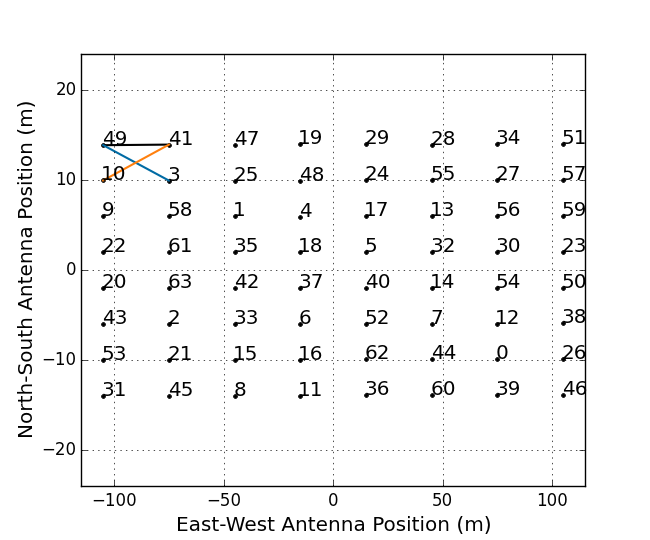
\includegraphics[width=1.85\columnwidth,height=\columnwidth]{plots/antenna_positions.png}
\caption{Antenna positions for the PAPER 64 observation run.}
\label{fig:antenna_positions}
\end{figure*}


\section{Analysis}
XXX FLOW CHART FIGURE XXX
We now describe the analysis pipeline leading up to the final power spectrum
measurement of our data set. To begin, we run a compression algorithm to reduce
the data volume of our raw data. This step, described in the appendix of
\cite{parsons_et_al2014a}, reduces data volume by a factor of 40. We then
calibrate on the basis of redundancy before using self-calibration
to solve for the absolute phase and gain parameters. After suppressing
foregrounds with a wide-band delay filter, we average the data in local
sidereal time. Finally, we apply a frine rate filter to optimally combine the
time domain data and use optimal quadratic estimators to make our estimae of
the 21 cm power spectrum.  Figure \ref{fig:analysis_pipeline} shows a block
diagram of the analysis pipeline and includes some information on simuations
and signal loss.

\subsection{Calibration}
\subsubsection{Redundant Calibration}
%    -Principles of redundant calibration. Fact that there is no signal loss in
%       this kind of measurement.
%       --PAPER has a redundant configuration. Therefore the number of baselines
%         is larger than the number of unique baselines in the array. There are
%         multiple baselines that measure the same sky.
%       --Introduce uniqe baseline. We define a unique baseline to be the set of
%         redundant baselines of a unique orientation.
%       --All baselines of a unique baseline measure the same sky and
%         therefore, differences between them are what need to be calibrated
%         out. These are the gain variations imparted on the incoming signal by
%         the antenna.
%       --There is no signal loss in this method. Sky signal is the same for
%         each of the redundant baselines is the same and hence any algorithm that
%         preserves common mode signal (which is what redcal does) is necessarily
%         lossless. This is an important point!  
%       --In addtion, because gains are normalized to have a unity magnitude the
%         input arn output flux scale are the same. (This is an omnical thing)

PAPER is arranged in a highly redundant configuration and thus lends itself to
use the redunancy in baselines for a relative calibration. Every instance of a
baseline of a given unique baseline type, for example the baseline 1-4 belongs
to the one column spacing and no row spaceing unique baseline type, measures the
same sky signal. On this basis, all of the differences between baselines of a
given unique baseline type are attributed to differences in signal chain, which
include variations in antennas, cables, and receivers, and should be calibrated
out. Redundant calibration inherently preserves common mode signal between
redundant baselines, and therefore this type of calibration is necessarily
lossless. 



%         
%    -What can we solve for and what can't we solve for. We can solve for the
%     relative complex gains between antennas, but not the absolute gain and phase.
%       --Because redundant calibration does not fold in any outside
%         information about the sky that we are observing, it inherently is a
%         relative calibration scheme that solves for the relative gains and
%         phases of antennas within the array. 
%       --Therefore, we cannot solve for the absolute phase and gain of the
%         array. There is not enough information.
%       --Absoulte phase and gain calibration are addressed in later sections.
Redundant calibration is a relative calibration procedure, hence we can only
solve for the relative complex gains between antennas. Redundant calibration
does not set anabsolute phase or gain scales due to the fact that it only
knows about other antennas, not absolute sky. Hence, there needs to be a second
round of calibration which folds in information about the sky to solve for the
absolution phases in order correctly phase to sourcese on the celestial sphere.

%
%    -Summary of the procedure of redundant calibration. This should be mixed in
%     with the equations from Zheng et. al.
%       --Two flavors of redundant calibration : logcal and lincal. Cite
%         liu,zheng.
%       --logcal takes log of equation 3 in zheng et. al., and thus becomes a
%         linear system. Can then solve for the log of the antenna gains, as
%         well as the true visibility of the sky as measured from a unique
%         baseline. 
%       --lincal is the linearization via taylor expansion of the same equation
%         3. This provides us with a better solution. The reason for doing
%         lincal is that logcal is a biased estimator. 
%       --Because there are more baselines than the number of unique baselines, 
%         we have an overdetermined system of equations and therefore can
%         uniquely solve for all of the gains and "true" visibilities.
Practiaclly, redundant calibration takes on two flavors, log calibration (logcal) and
linear calibration (lincal) (\cite{liu_et_al2010,zheng_et_al2014}). Logcal, takes
the logarithm of the visibility measured by an interferometer (equation 4 of
\cite{zheng_et_al2014}) to give a linearized system which can then be fit to
using linear least square. We end up fitting 
\begin{equation}
    \log{v_{ij}} = \log{g_{i}^{*}} + \log{g_{j}} + \log{y_{i-j}},
\end{equation}
where the $g_{i}$'s are the
complex gains of each antenna and $y_{i-j}$ is the visibility of the given
baseline if it measured the perfect sky. Redundancy gives us an overconstrained
system of equations and we can thus solve for complex gains from each antenna.
In addition we also get a model visibility of for a given given baseline.
Averaging these models together for redundant baselines gives us a an estimate
of our model visibility for a given baseline type.

Lincal taylor expands the visibility around some initial estimates of the gains
and model visibilities.  The benefit of lincal is that it is not a biased
estimator as opposed to logcal which takes the logarithm of additive noise.

%    -How was this calibration applied to the data. 
%       --Using omnical package. Give credit jeff and url to omnical. Cite
%         paper.
%       --Implements both logcal and lincal. Discuss the speed ups. 
%       --gains were applied to the uv datasets and written out in the same
%         format. However, Omnical is quite general and solutions can be written
%         out in text files and adapted to other file formats.
%    
%    -Removing additive offset and what is the time cadence of all of this.
%       
%    -Diagnostic figures : Chi-squared, complex plane, stability vs. time and
%                          frequency.

Implementaion of redundant calibration was done with the ${Omnical}$ package, an
open source redundant calibration package written by Jeff
Zheng \footnote{https://github.com/jeffzhen/omnical}\cite{zheng_et_al2014}. This
package implements both logcal and lincal with an incredible speed up from
the previous homegrown routine used in \cite{parsons_et_al2014a}. 


XXXadd in duscussion about removing additive offsets and time cadence of
that)XXX.

\subsubsection{Absolute Phase Calibration}
%    -Selfcal to pictor, fornax, and crab (to get the north-south components).
%       --Reiterate that redundant cal does not solve for the overall flux and
%         phase parameters. 
%       --There are two final phase parameters we must solve
%         for in order to correctly phase to a source on the sky. Redundancy
%         only gets you so far, but still need to be able to unambiguously phase
%         to sources.
%       --We use self calibration to solve for the global phase parameters using
%         Pictor A, Fornax A, and Crab Nebula. 
%       --
%
%    -Diagnostic Plots: Show Field image from Bernardi. This will give
%     confidence in a good absolute phase calibration.

After solving for the relative phases and gains of the antennas using redcal, an
overall phase and gain calibration needs to be solved for. We use the standard self
calibration (selfcal) method for radio interferometers in order to solve for
these over all parameters. The absolute phase calibration was solved for using using 
Pictor A, Fornax A, and Crab Nebula. Figure \ref{fig:field_image} shows an
image of the field with Pictor A (5:19:49.70, -45:46:45.0)  and Fornax A
(3:22:41.70,-37:12:30.0). The measured source positions are the same as the the
catalogue positions for these sources.XXX make sure of this statementXXX

\subsubsection{Absolute Gain Calibration}
%    -Calibrated to Pictor A. 
%       --As before, redundant calibration cannot set a global flux scale. For
%       our measurements to be correct, we need to set a fluxscale. We use
%       Pictor A to set our fluxscale. Cite Dannys pictor paper.
%      
%    -Our bandpass model is a 9th degree polynomial. 
%       --In order to set our fluxscale, we beamform our data upto pictor A,
%         summing baselines, and then then fit a 9th degree polynomial to the
%         bandpass. This is our measure of the spectrum of Pictor A. 
%       --Because we are beamforming to pictor and fitting a polynomial to the
%         bandpass, there is signal loss. This signal loss is of the 
%    -Tabulate signal loss due to this model. Averaging over Nbls, times gives us
%     an average over independent uv modes.
%       --Working on this... a few questions about it.
%
%    -The actual signal loss on a given mode is L/N where L is the loss for a
%     single instance of the beamform (one time, one baseline) and N is the
%     number of baseline and times that were summed.
%
%    -PLOTS: 
%        --A plot that is the phased to pictor beamform gain 
%          (or maybe just a single channel for all days.
%        --The measured and theoretical pictor spectrum 
%        --A comparison to the PSA32 Flux CAL.













%These lists were My bullet points.
%\begin{itemize}
%    \item{Overview of the calibration with emphasis on Omnical.}
%    \item{Rough Calibration : Can cite Parsons 2014 for the details.}
%    \begin{itemize}
%        \item{Discuss the first pass of redundant phase and gain calibration.
%              Absolute phase calibration using pictor, fornax and crab in the
%              fit.}
%        \item{Absolute flux scale using Pictor A. Want to address signal loss.
%             Maybe delay the issue of signal loss to a "Signal Loss" section
%             which takes into account the signal loss in various stages of the 
%             analysis?}
%        \item{Add in details of the loss of eor signal. Do simulations to get
%              numbers. }
%        \item{Plots : Measured pictor spectrum with comparison to the Danny
%              pictor spectrum. Maybe some simulation plots showing the signal
%              loss due to the polynomial fit to pic spec.}
%    \end{itemize}
%    \item{Omnical}
%    \begin{itemize}
%        \item{What is omnical?}
%        \item{Why are we using it? To get a frequency/time dependent
%calibration. Need to address why this is not overfitting. That is why is this
%just not flatting everything out.}
%        \item{Address non-possibility of signal loss.}
%        \item{Refresh formalism (do this here or in the intro of calibration?)}
%        \item{What is it doing? logcal/lincal. Chi-squared and how that
%              determines the goodness of the fits to the model baselines. What
%model are we using? Is it a good model?}
%        \item{Plots: Chi-squared plots. Compex plane plots that show
%              improvements over uncalibrated/rough/omnical calibrated. 
%              Time and frequency stability.}
%    phase to pic gain, pic spec, comparison to psa32.
%    \end{itemize} 
%\end{itemize}

%OLD TEXT START
%\subsubsection{Overview}
%As the name suggests, redundant calibration (\cite{liu_et_al2010},
%\cite{zheng_et_al2014}) uses redundancy within the array to solve for relative
%phases and gains of the antennas. To explain redundant calibration, suppose that
%the baseline between antennas $i,j$ measure a visibility $v_{ij}$, then we have 
%
%\begin{equation}\label{eqn:redcal}
%    v_{ij} = g_{i}g_{j}^{*}y_{i-j} + n_{ij},   
%\end{equation}
%where $g_{i}$,$g_{j}$ are the complex gains due to antenna $i$ and antenna $j$,
%respectively, $y_{i-j}$ is the true visibility measured by perfect antennas
%$i$,$j$ for the given baseline type, and $n_{ij}$ is the residual noise from
%the baseline.  If the number of baselines of a given type is much greater than
%the number of baselines types this problem is over constrained and $g_{i}i$,
%$g_{j}$, and $y_{i-j}$ can be solved for. PAPER is in this limit due to the
%maximally redundant configuration as shown in figure \ref{fig:antenna_pos}. 
%
%Redundant calibration comes in two flavors: log calibration and linear
%calibration. Log calibration, or logcal for short, takes the logarithm of
%equation \ref{eqn:redcal} to give a linearized system. Hence, solutions can be
%solved for by using standard linear algebra techniques. However, this method is
%biased. On the other hand linear calibration, or lincal for short, is an
%unbiased method of solving for the complex gain solutions. In this method
%equation \ref{eqn:redcal} is Taylor expanded about an initial guess for the
%$g_{i}$'s and $y_{i-j}$'s to give a linearized equation which can be used to
%solve for the complex gains and sky model. 
%
%In this analysis we used a logcal algorithm based in delay space to get a rough
%calibration of the dataset. This was followed by an absolute calibration to set
%the overall phase and flux scale using a self calibration. We used model phase
%centers of Pictor, Fornax A, and Crab Nebula. The absolute amplitude is set
%by the flux of Pictor A found in \cite{jacobs_et_al2013}, whose spectrum is
%defined by 
%\begin{equation}
%    S_{\nu} = 382(\frac{\nu}{150 MHz})^{-.76} Jy.
%\end{equation}
%
%Finally, we used the Omnical calibration package to do another round of
%redundant calibration to get even more accurate calibration parameters.
%
%\subsection{logcal-for lack of a better title}
%We first perform the same calibration that was
%done in \citep{parsons_et_al2014a}. That is, we use redundancy to do a relative
%phase\footnote{In actuality, we solve for delays to get around phase wrapping
%issues. These delays are applied to visibilities as $e^{2\pi{i}\tau\nu}$}
%calibration between antennas, which removes the electrical delays from cables in
%the signal path. Due to redundancy, we can calibrate out all of the per-antennas
%delays in the signal path relative to two delay parameters which we call
%$\tau_{ns}$ and $\tau_{es}$. These delays are the relative electrical delays
%that correspond to baseline delays in the north-south and east-west component
%for 2 reference baselines (49-10 and 49-41,respectively). These solutions were
%then applied to the data set which was calibrated again with Omnical. 
%
%The application of this calibration to the data set before Omnical was needed
%because in order to calibrate accurately, Omnical needs to have a rough estimate
%for the calibration solutions for every antenna. In \cite{zheng_et_al2014}, a
%model of the sky was used in order get the rough estimate of the solutions.
%Here, we use actual sky data to get the rough calibration. Because the solutions
%are derived from the instrument, we can incorporate into the solutions antenna
%based variations. 
% 
%The antenna based
%delay solutions vary as much as a couple nanoseconds day to day when solutions
%are averaged over hour long timescales withing a day. However, the variations in
%solutions is worse when only averaging over ten minute time scales. Therefore
%need for better calibration is requred.  We use self calibration to derive the
%two unknow parameters, $\tau_{ns}$ and $\tau_{ew}$, by using the Crab Nebula,
%Fornax A, and Pictor A.
%
%Note that there is no possibility of signal loss (see \citep{parsons_et_al2014a}).
%
%\subsection{Gain Calibration}
%Gain calibration was derived on the basis of redundancy and self calibration.
%The phase calibrations described above, simultaneously also calibrated for the
%relative gain variation between antennas. Again we can only calibrate to a fiducial
%antenna (49) whose gain is defined as unity. We then perform a self calibration
%to set the flux scale to Pictor A whose spectrum is derived in
%\citep{jacobs_et_al2013}. We use the same methods describes in \citep{parsons_et_al2014a}.
%
%Figure \ref{fig:bmfom_pic} shows that dataset beamformed to Pictor A, with log
%janskies on the y axis and lst on the xaxis for a frequncy of .1 + (120/203)*.1/203. 
%As can be seen, the day to day variation in the formed beam has a fractional
%spread of about 10$\%$.  This shows the stability of the instrument and the well
%behaved calibration solutions derived above. 
%
%\subsection{Omnical}
%(How did we know that our calibrations were not good enough? Because of the power
%spectrum? PSA32? We did beamform data to pictorA and say that vs LST, the
%beamform matched well day to day with a fractional spread of about 10$\%$) 
%
%The complex gain solutions found in the previous calibration pipeline were
%averaged together in time and one solution per frequency was used for the array.
%This jived with the philosophy that the array was stable in time and frequency.
%However, upon further review of this data set, it seemed more and more likely
%that this was not the case anymore. (Is this even true? What specifically? Think
%Man!) 
%
%Due to clues that showed that our data set had time dependent calibration
%solutions, it was imperative that we do a better job at calibrating our array.
%
%The Omnical redundant calibrator
%package\footnote{https://github.com/jeffzhen/omnical} (omnical) performs
%redundant calibration for every time and frequency in a dataset using both
%logcal and lincal methods as described in \cite{zheng_et_al2014}. It also
%contains methods on the quality of the solutions by providin a chi-square for
%the fits to the data. 
%
%For this dataset, omnical first performed a logcal (again) to attain a solution
%per time and frequency. This solution was passed to lincal which iteratively
%solved for the complex gain solutions. The convergence criteria was when the
%$\chi^{2}$ decreased by less than $.01\%$. The $\chi^{2}$ for the fit used in
%Omnical is given by 
%\begin{equation}
%    \chi^{2} = \sum_{ij}|v_{ij} - y_{i-j}g_{i}^{*}g_{j}|^{2},
%\end{equation}
%
%which differs from normal nomenclature because we are not inverse varaince
%weighting. Note that this $\chi^{2}$ is summing over all baselines and hence 
%giving more weight to higher gains. Note that omnical fits for each of the
%complex gains and the model visibility, $y_{i-j}$,  for a unique baseline.
%Using this information, figure \ref{fig:chi_2} shows that the $\chi^{2}$ is close
%to 1 for all channels and time (for this day of data). need noise model for
%this.
%
%Figure \ref{fig:gain_solutions} shows the gain solutions output by omnical. The
%amplitude of the gains are roughly order unity through out. These are relative
%gains between antennas and hence the over flux scale set to Pictor A is still
%valid. The absolute calibration is still valid. 
%
%Since Omnical outputs a model visibility of what a unique baseline should
%measure, which is derived from the data by removing all of the variation between
%unique types of baselines and averaging, we are able to use these outputs as our
%dataset. Infact, this is what is done. 
%%waterfalls of chi squared and solutions.
%%day to day repeatability.
%%The output of the omnical - 
%%
%OLD TEXT END



\subsection{Wideband delay filtering}
%   -Can cite Parsons 2014a
%       --We use the same wbd filter as in Parsons 2014a. That is we do a per
%         baseline delay filtering with a buffer of 15 nanoseconds. 
%   -Quantify signal loss. 
%       --I think this is the same as before. Since delay filtering is done on a
%       per baseline basis, the signal loss from the previous paper and this one
%       is the same. We are using the same filter.
%   -PLOTS:
%        --waterfalls of before and after cleaning.
%        --signal loss vs. k_parallel

For a detailed description of delay filtering, we refer the reader to
\cite{parsons_backer2009}. In this analysis we use the same wideband delay
filter as described \cite{parsons_et_al2014a}, namely the horizon limit for a
given baseline plus a 15 nanosecond buffer to account for leakage of foregrounds
outside of the horizon. We note that since delay filtering is applied on a per
baseline basis, the signal loss associated with this type of filter is the same
as in \cite{parsons_et_al2014a}. We reiterate the results here: there is a 4.8\%
signal loss for the first mode outside of the horizon, 1.3\% for the next mode
out, and less than .0015\% for the higher modes.


\subsection{RFI and Crosstalk mitigation}
\begin{itemize}
    \item{Discuss, briefly, RFI and Crosstalk removal. Note that this happens
after foreground removal. Possibility of signal loss?}
\end{itemize}

After the wideband delay filter, we conduct another round of RFI and crosstalk
removal which was overshadowed by the foreground signal. For RFI excision we
apply a median filter which flags above $3\sigma$. Foregrounds kept us using the
traditional method of removing cross talk which consisted of subtracting hour
long averages from each visibility. This was due to the fact that some days in
the observation had gaps in time owning to some technical difficulties during
observations. However, with foregrounds removed we were able to remove 10 minute
averages from every visibility within a file (files have a cadence of ten
minutes). Normally, hour long averages are needed for foreground contained data
to wash out the fringes from the said foregrounds to detect the static phase
bias that is crosstalk. For foreground removed data, we do not have this
complication since bright foregrounds are not dominating the average and are
able to remove the offset by subtracting shorter sums.

\subsection{Stokes I : cite Moore et.al.}
%We form stokes I = .5 (xx + yy)
\subsection{LST Binning}
%   -Practicals: bin size, number of days, range of days 
%       --We LST bin the data over the 120 night data set into time bins of
%         42.95 seconds. 
%       --WE form multiple LST data sets which bin different days throughout the
%       observation together. These datasets help us remove systematics in the
%       power spectrum estimation. They also provide us a way to jackknife the
%       data set.
%   -N lst data sets. Jack-knifing etc.
%   -Median Filter : no signal loss. Filtering because of outliers in time that
%    find their way into the data 
%       --While lst binning, we apply a median filter which for a given lst and
%       frequency bin, removes data which falls outside 3 sigma of the median of
%       the dataset. This filtering is necessary, because of the non gaussian
%       events that crept their way into the data set, such as RFI, etc...
%       --There is no signal loss associated with this because we are using
%       median statistics. 
%   -Plots: Integration counts vs. LST/freq  waterfall.

Once smooth sources have been removed and a final pass of RFI excision and
crosstalk removal have been performed, the data is averaged in local sidereal
time (LST) with bins of width 43 seconds to match the integration time of the
data. The data set consisted of 135 unevenly sampled days with the effective
number of total days being 123.57. This uneven sampling in the data set was due
to technical difficulties in the recording of disks.

Sporadic RFI events can skew individual LST bins away from the median value of
the sky at a given LST. Therefore, we compute the median in a given LST bin for
each frequency and flag off data that is 3 sigma outside of that median before
averaging. This filter mitigates the adverse effects of RFI from dominating a
LST bin. 

%\subsubsection{A noise study}
%During the LST averaging, we compute the median and the variance for every LST
%and frequency bin. The variance in particular is of importance becuase it allows
%us to estimate the system temperature, $T_{sys}$, as a function of LST and
%frequency. The variance is computed, per frequency, for all the visibilities
%that are included in a given LST bin, which gives us an estimate ${I_{rms}}$,
%the specific intensity in Jy, which is then converted to a $T_{rms}$ in the
%usual way, 
%\begin{equation}
%    T_{rms} = \frac{I_{rms}\lambda^{2}}{2k\Omega}.
%\end{equation}
%
%where $\lambda$ is the observing wavelength, $\Omega$ is the size of the beam in
%steradian, and $k$ is the boltzmann constant. We convert $T_{rms}$ to a system
%temperature by scaling up the rms with the effective integration time and
%bandwidth used. That is, 
%\begin{equation}
%    T_{sys} = T_{rms} \times \sqrt{\Delta{B}t_{int}}.
%\end{equation}
%
%Figure \ref{fig:tsys_lst_fq} shows the system temperature as a function of
%LST and frequncy. In our "cold" patch, we find that $T_{sys}$ is around $500K$.
%
%
%\begin{figure}
%\centering
%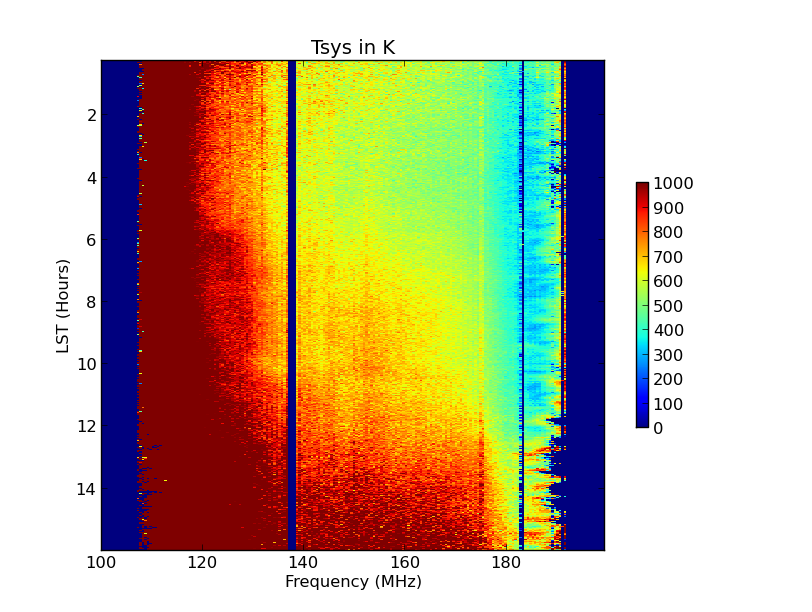
\includegraphics[width=\columnwidth]{plots/tsys_lst_freq.png}
%\caption{Tsys as a function of lst and frequency. The cold spot resides in the
%lst range of 1-7hours.}
%\ref{fig:tsys_lst_fq}
%\end{figure}






\subsection{optimal Fringe-rate filter}
%   -What is fringe rate filtering. Cite Parsons And Liu 2014.
%       --Fringe Rate filtering is nothing more then a time domain weighted
%         average per frequency of of visibilities. The filter can be applied 
%         as either a convolution in the time domain or a multiplicative fourier
%         filter in fringe rate space. 
%       --We first calculate fringe rate filter such that we upweight the more
%         sensitive fringe rates versus the not so sensitve fringe rates by
%         weighting the fringe rates for a given baseline by its beam.
%   -Effective beam areas.
%       --When fringe rate filtering, we are upweighting fringe rates that
%         are most sensitive. That is we are weighting these fringe rates by the
%         beam of a baseline. This has the effect of narrowing the effective
%         beam. It turns out that we are removing more noise than signal,
%         because we are essentially keeping the most sensitive parts of the
%         sky. This actually gives us a sensitivity boost of about a factor of
%         2. 
%   -effective integration time and number of modes. 
%       --Do calculations.
%       --Fringe rate filtering is effectively a weighted average in time and
%       thus there is an effective integration time. We can calculate this
%       integration time by noting that power (or variance) is a conserved
%       quantity. Therefore, comparing the integral of a variance=1 noise signal
%       when it is fringe rate filtered to when it is not, gives us a fractional
%       integration time. 
%           \frac{ \int_{t_{start}}^t_{end}{\sigma^{2}*F_{constant}(t)dt
%           }}{\int_{t_{start}}^t_{end}{\sigma^{2}*F_{filter}(t)dt = fraction.
%            t_int = fraction * t_start-t_end
%           Something like that.
%       --Due to the fact that fringe rate filtering is effectively averaging in
%         time, A fringe rate filter reduces the number of independent modes on
%         the sky. The number of modes in an entire day drop just 45
%         (24hrs/1900sec)  independent modes on the sky. 
%   -PLOTS: 
%       --FR filter (both in fr and time space), applied to data.
%       --Beam after fringe-rate filter. 
%       --Waterfalls.
%       -- apply filters to foreground data. Compute fr of pica and show that we
%          are not killing the sky.
%   
%   code to get the integration time of fringe rate filter. This is 1894 for channel 100
%   beam_w_fr = frf_conv.get_beam_w_fr(aa, (1,4))
%   t,firs,frbins,frspace = frf_conv.get_fringe_rate_kernels(beam_w_fr, 42.8, 401)
%   fr100 = frspace[100]
%   t_int = 42.8/n.mean(fr100)
%   

Before forming power spectra we need to time average visibilities that measure
the same $k$ mode on the sky. This is the best way to combine data because we
get a $\sqrt{N}$, where N is the number of samples, gain in sensitivity. This is
in oppostion to weighting after forming power spectra, where noise beats down as
the $\sqrt{N}$. Rather than a straight averaging in time, we can do better by
using a weighted averge. Specifically, we want to upweight samples that have
higher signal-to-noise. 

This is acheived by applying a carefully crafted filter in fringe rate domain,
the fourier dual to time. Different patches on the sky correspond to different
fringe rates, for a given baseline and frequency. Maximum fringe rates are found
along the equatorial plane where zero fringe rates are found around the poles
(sources at the poles do not move through the fringes of a baselines). Sources
on the other side of the pole, corresponds to negative fringe rates, because
they move through the fringe pattern in the opposite direction. By weighing the
fringe rates sampled by a baseline by the beam response of the baseline, gives
us the optimal fringe rate filer to use for time averaging. See Parsons/Liu 2014
for a detailed discussion.

We implement the optimal fringe rate filter by first calculating the fringe rate
of everypoint on the sky and weighting it the beam of a given baseline, summing
along constant fringe rate contours. Note that because the data already has one
factor of the power beam in it, we only need to weight the fringe rates by the
power beam and not square it. That is we are upweighting fringe rate bins that
have greater signal-to-noise.  We then fit a gaussian to the optimal filter to
have a smooth function, along with tanh function for to have a smooth cut off
at the maximum fringe rate for the given baseline and frequency.  Note that
this only calculated for a given frequency and scaled to other frequencies, due
to the fact that fringe rate scales linearly with frequency via

\begin{equation}
    f_{max} = \frac{|\mathbf{b}_{eq}|}{c}\omega_{\oplus}\nu
\end{equation}


We then fourier transform the omptimal fringe rate filter and multipy by a
blackman-harris window function. This convolution kernel is then applied to 
visibilities for every baseline at every frequncy. We implement the fringe rate
filter over the span of 17163 seconds even though the full with half max of the
filter spans ~15 minutes for a 30 meter baseline. This 

Since the PAPER beam is ~45 degrees, and the array is located at a declination
of $-30^{\circ}$ the fringe rates associated with the low signal to noise (down
in the beam) correspond to very high and very low/negative fringe rates. Figure
\ref{fig:fringe_rate_cut} shows a cut of the optimal fringe rate at XXXMHz for a 30
m east west baseline. Therefore, the implemented fringe rate filter removes some
sky signal, signal associated with fringe rates outside of the ranges shown in
Figure \ref{fig:fringe_rate_cut}. Figure \ref{fig:fr_preserved_signal} shows
that the applied filter removes sky associated with negative fringe rates and
very high fringe rates. 

\begin{figure}
\centering
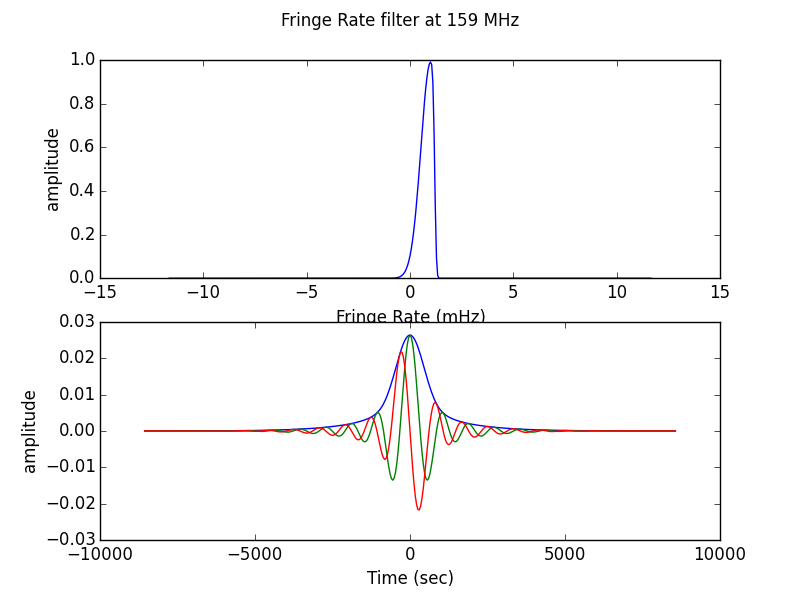
\includegraphics[width=\columnwidth]{plots/fr_filter_slice.png}
\caption{slice of a fringe rate filter at a frequency of 159MHz. Top is the
filter in fringe rate domain. The bottom consists of the corresponding time
domain filter gotten by fourier transforming and windowing with a
blackman-harris window to damp the tails.}
\label{fig:fringe_rate_cut}
\end{figure}

\begin{figure*}[t!]\centering
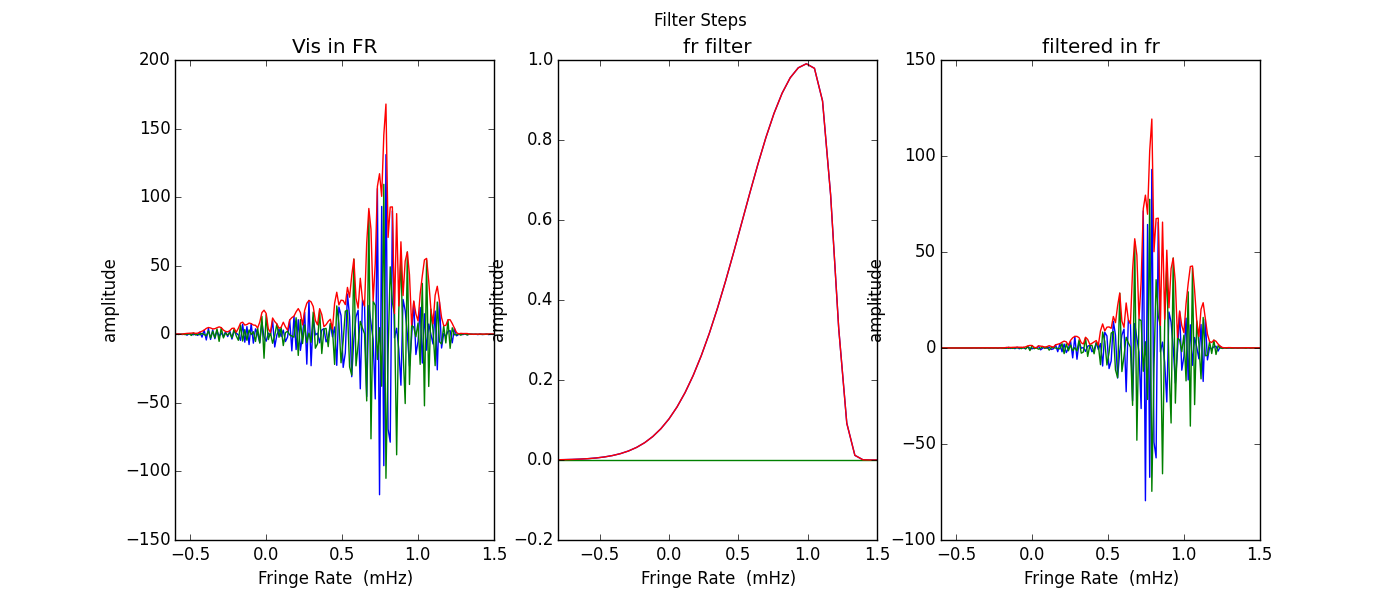
\includegraphics[width=2\columnwidth]{plots/fr_preserved_signal.png}
\caption{slice of a fringe rate filter at a frequency of 159MHz. Shown here is
the fringe-rate transform of foreground contained data for a 30 m east-west
baseline. Blue and green are the real and imaginary part, respectively and red
is the absolute valeu. Note the maximum and minimum fringerates correspond to
the theoretical minimum and maximum for a baseline of this length at 159 MHz.
The center panel shows the real (red)  and imaginary (green) parts of the fringe
rate filter to be applied. Finally, the last panel on the right shows that the
fringe rate filtered visibilities. The fringe rate filter is just a weighting
applied in fringe rate space and retains foregrounds.}
\label{fig:fr_preserved_signal}
\end{figure*}

%\begin{figure}[h!]\centering
%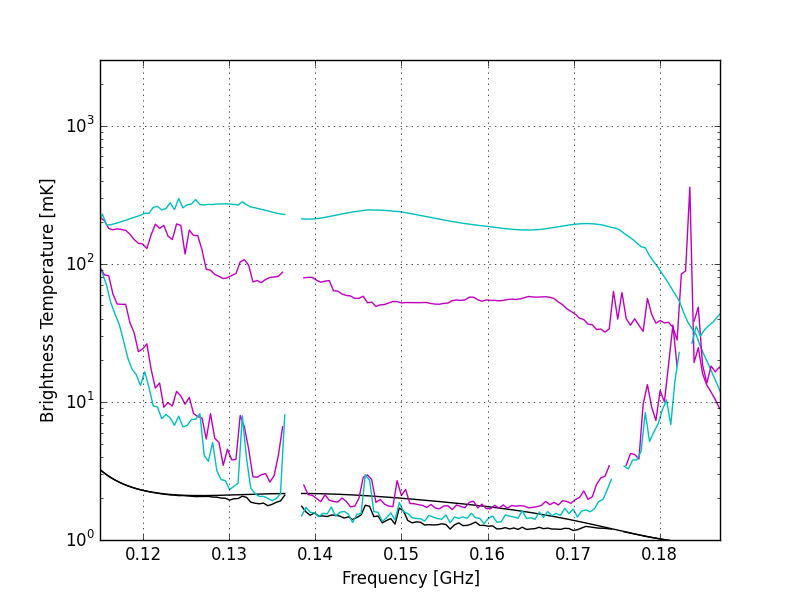
\includegraphics[width=\columnwidth, height=.8\columnwidth]{plots/noise_t_35.png}
%\caption{Estimates of noise temperature. Magenta is frequncy differenced
%estimate where the cyan is the time differenced estimate. All curves are
%averaged over all 30m east-west baselines (56) and averaged incoherently in 43s
%bins of LST from LST 3 to 5 hours with a channel bandwidth of 490 kHz.}
%\label{fig:noise_t}
%\end{figure}


%\begin{figure}[h!]\centering
%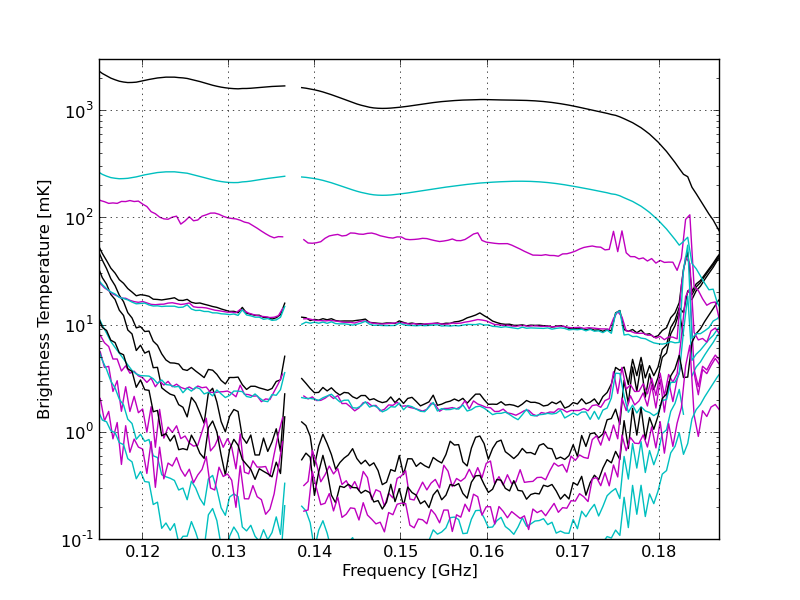
\includegraphics[width=\columnwidth, height=.8\columnwidth]{plots/noise_vs_fq_plot.png}
%\caption{Estimates of noise temperature. Magenta is frequncy differenced
%estimate where the cyan is the time differenced estimate. Averaged in LST from 3
%to 5 hours. on uv files calibrated with omnical. fg,delay filtered, baseline
%averaged, normal fringe rate filter, optimal fringe rate filtering.}
%\label{fig:noise_omni_uv}
%\end{figure}


\subsection{Optimal Quadratic Estimator and Covariance}
%   -Motivate method with discussion of empirical estimate of covariances and
%    problem of limited modes.
%       --Because we dont know the true covariances between baselines and
%         channels we have to estimate the covariances epirically from data. 
%       --We do this by taking the outer product of our data vector (consisting
%         of a visibilies for every baseline of a given unique baseline type).
%         The outer product is calculated per time sample, thus we average over
%         a "clean" (what do i mean by this?) lst range.
%       --Hence, the quality of the estimate of the covariances between
%         baselines depends on the average in time ( the ensemble average). 
%       --The fact that we do not know what the full covariance matrix looks
%         like leads to signal loss. We have an estimate of the covariance, not
%         the true covariance matrix. There is no way to truly know what the
%         covariance matrix is for our data set. 
%       --After fringerate filtering, the number of independent modes on the
%         decreases substantially because we are averaging over 1900 seconds
%         ~=31.67 minutes. Therefore the number of independent modes decreases
%         1900/(the beam in time). 
%       --In our range of lsts used, we only have roughly 20 independent
%         samples. Therefore we end up with an ill determined covariance matrix
%         to describe our data. 
%       --In addition, because of the highly redundant nature of the array,
%         the covariance matrix is highly singular and therefore not invertible.
There are inherent covariances in the data between baselines and frequencies.
Figure \ref{fig:covariances} shows these covariances estimated empirically from
the data itself. This estimate is the outer product of our data vector with
itself and in our case, this averagse per baseline visibilities of a unique type
over time. Hence, the quality of the estimate of the data covariance matrix
depends on the number of independent modes we are averaging over. After
fringe-rate filtering, the number of independent modes  decreases significantly
leaving us with only ~20 independent measurements of the sky. This reduction in
modes leads to a noisy estimate of the covaraince matrix. This leads to a
broader problem in this type of analysis: the fact that we estimate our
covariances from the data and do not know the true covariance matrix itself,
leads to signal loss. Knowing the true covaraiance a data set requires complete
knowledge of the instrument and the sky. 



%
%   -Mathematics compared to ideal optimal Quadratic Estimator.
%       --In the quadratic estimator formalism, the value of the power spectrum,
%         $p_{\alpha}$  in the $\alpha^{th}$ bin is given by
%         $Mq_{\alpha}=$Mx^{\dagger}C{-1}Q_{\alpha}C^{-1}x, where x is a vector
%         containing the binned data in frequency domain, $x = V(\nu)$, C is the
%         estimate of the covariance matrix of of our data, C = <xx^{\dagger}>,
%         $Q_{\alpha}$ is defined such that $Q_{\alpha}=\frac{dC}{d\alpha}$, and
%         M is a normalization matrix that normalizes the estimator.
%       --Generally, the covaraince matrix used is the full covaraince between
%         all baselines and channels. 
%       --Because of redundancy, the matrix is singular and not invertible. We
%         therefore construct a pseudo inverse for C. In addtion to the psaudo
%         inverse we take only the auto-baseline covarainces, masking out the
%         covariances between baselines. This, is invertible. WE can thus apply
%         the inverse of C in the above equation.
%
%   -Counting of independent modes.
%       --Number of independent modes = 2*#of lst hours used in analysis. This
%         is because 1900 seconds ~ 30 minutes.
Here we briefly review the optimal quadratic esitimator (OQE) formalism with an
emphasis on application to our data. The end goal is to make an estimate of
the 21 cm power spectrum, $P(\k)$, defined such that 

\begin{equation}
\label{eqn:pspec_def}
    \expval{\tilde{T}_{b}(\k)\tilde{T}^{*}_{b}(\k^{\prime})} =
            (2\pi)^{3}\delta^{D}(\k - \k^{\prime})P(\k). 
\end{equation}
For a data vector $\x$, the optimal quadratic estimator is given by 
\begin{equation}
\label{eqn:quad_est}
    \hat{q}_{\alpha} = \frac{1}{2}\x^{t}\mathbf{C}^{-1}\mathbf{Q}_{\alpha}\mathbf{C}^{-1}\x - b_{\alpha},
\end{equation}
up to some normalization matrix $\mathbf{M}$. With the normalization mtrix, the
estimate of the power spectrum in bin $\alpha$ is given by
\begin{equation}
    \hat{p}_{\alpha} = \mathbf{M}\hat{q}_{\alpha}, 
\end{equation}
where $\hat{p}_{\alpha}$ is the estimate of the power spectrum.
In our analysis, $\x$ is the set of visibilities for the redundant baselines of
a single column east-west spacing for a frequency spanning 10 MHz centered at
151.5 MHz. To first order we estimate our covariance matrix by taking the outer
product of our data vector with itself, $\mathbf{C} = \expval{\x^{t}\x}$,
collapsing over the time axis. We discuss the consequences of the covariance
matrix later in this section.  $\mathbf{Q}$ is defined as the derivative of
$\mathbf{C}$ with respect to $\alpha$. The $\mathbf{Q}$ matrix encodes the delay
transform to go from frequency domain to delay domain, where $P(k)$ can be
estimated. Finally, $b_{\alpha}$ is a bias to the estimate that needs to be
subtracted off. In our analysis, we are constructing an unbiased estimator and
therefore do not need to subtract this term. The normaliztion matrix is defined
such that
\begin{equation}
    \mathbf{W} = \mathbf{M}\mathbf{F}, 
\end{equation}
where $\mathbf{F}$ is the Fisher information matrix, given by $F = cov(\hat{q})
= 2tr(C^{-1}Q_{\alpha}C^{-1}Q_{\beta})$ and $\mathbf{W}$ is 
the window function matrix. The window functions measure the degree to which
power from $k$ bins couple into the measurement of the power measured in the
$\alpha$'th bin.

%   -Cholesky Decomposition and window functions.
%       --The optimal window functions (that minimize the vertical error bars of
%       the estimate, are given by the inverse of the Fisher matrix. However,
%       there is a trade off such that this incorporates information from all of
%       the k-modes. 
%       --Some other choices of the window functions are the square root of the
%       fisher matrix or the identity. 
%       --We use the cholesky decomposition of the Fisher Matrix such that we
%       can write F = LL^{\dagger}, where L is a lower triangular matrix. This
%       is possible for any hermitian positive-definite matrix.
%       --We use L for our window functions because for every k-bin, it does not
%       use information from the k-bins below it. And thus there is no mixing of
%       modes lower than it. 
%       --This is particularly important because it doesn't insures that there
%       is no leakage of the modes within the horizon to modes outside of it.         
%

The choice for the normalization matrix is up to the analyst. Picking
$\mathbf{M} = \mathbf{F}^{-1}$  minimizes the error bars in the final power
spectrum estimate with the trade off that the estimate of the power spectrum in
the $\alpha$'th bin is coupled with every other measurement in other bins. Even
though this choice gives us the smallest error bars possible, we opt for a
different choice of window function. We first take the Cholesky-decompositon of
the Fisher matrix such that $\mathbf{F} = \mathbf{L}\mathbf{L}^{\dagger}$, where
$\mathbf{L}$ is a lower triangular matrix. Then, we take ${\mathbf{M}} =
\mathbf{L}^{-1}$ to be our normalization matrix. Therefore, ${\mathbf{M}}$ is
still a lower triangular and the window function matrix is also block diagonal.
This choice of $\mathbf{M}$ has the effect on the final estimate of the power
spectrum in the $\alpha$'th bin of only coupling modes larger than the
$\alpha$'th mode are coupled in to the estimate.  Therefore, this has the
consequence of not coupling the modes inside to horizon in to measurments of the
power spectrum outside the horizon. Figure \ref{fig:window_functions} shows
these window functions.%XXX be more clear, and get the math right.

A few issues arise in our application of this optimal method. These issues have
various effects on our analysis choices. First, the input data is highly
redundant and hence the covariance matrix is singular and thus not invertible.
However, we consider a covariance matrix made up of the covariances of each
baseline with itself and mask of the covariance between baselines (see figure
\ref{fig:covariance_matrix}). This decreases the degrees of freedom available
and hence $\mathbf{C}$ becomes non-singular. Therefore, the weighting we apply
to our data does not take into account the covaraiance between baselines, only
the covariances between frequencies for a baseline. 


%
%   -Potential for signal loss.
%       --In a traditional OQE method, the process is lossless by construction.
%         Because we are tweaking this method, and the fact that we have non
%         gaussian systematics in our data, there is a potential for signal
%         loss. 
Secondly, our estimate of the covariance matrix by the limited
number of independent modes we observe in our data. Hence, there is a high
possibility of signal loss. In order to quntify the signal loss in our analysis,
we run simulations of an injected eor signal through our pipeline. This will be
discussed further below.


%   -Simulations
%       --In order to show the degree that there could be signal loss, we run
%         simulations to show that an EOR -like signal does pop come out in our
%         data. 
%       --We inject a common eor like signal, a complex random white noise
%         signal, on to all of the baseline data used in this analysisi for a
%         given time. This signal is fringe rate filtered to match the data and
%         therefore, the number of independent modes matches the input data. 
%       --We run this simulation for varying signal levels, showing that this
%         signal can infact be recovered, with some signal loss.
%       --These simulations show that there is signal loss in this method.
%         However, if the signal was bright enough, we would be able to see it.
%         Since we don't see signal in the actual data, we can say that we have
%         not detected the EOR signal yet.

In order to understand the degree of signal loss due to our empirical estimates of
the covariances, we simulate the injection of an eor model and measure the
signal loss associated with running the full covariance analysis. These
simulations consist of injecting a model eor signal on top of the the data and
running through our power spectrum estimator. In order to quantify this, we
subtract the final power spectrum from one that had no model injection to
measure the final injected signal power spectrum. Comparing this to the input
data gives us an estimate of the signal loss associated with our pipeline.

The eor model used in the simulations described consists of a sky modeled to
have a flat power spectrum in $P(k)$. We necessitate that the sky has this flat
power spectrum and work backward to derive visibilities that describe that sky. 
Some more detail here would be nice, giving credit to Carina. ... This signal is
then fringe rate filtered to match the data. Hence, the number of independent
modes in these simulations is the same as the data, which is ~20 independent modes.

Figure \ref{table:pspec_sig_loss} tabulates the signal loss associated with our
powerspectrum pipeline as a function of the input signal level. We tabulate this
as a function of $k$. 

\begin{table}[!h]
\caption{Table of signal loss associated with the power spectrum pipeline as a
function of the input signal level.}
\begin{center}
\begin{tabular}{|c|c|c|c|c|c|c|}
\hline 
a&a&a&a&a&a&a\\
\hline
\end{tabular}
\end{center}
\label{table:pspec_sig_loss}
\end{table}%




%   -Maybe : Problem of low noise measurements in this method of analysis i.e.
%    singular matrics - For Adrian.
%
%   -Boot strapping 
%       --In order to calculate the residual noise in our power spectrum
%         estimate, we bootstrap the baseline samples at the output of the
%         quadratic estimator. 
%       --Doing this gives us the variance of the power spectrum estimate and
%         thus derives the 2 sigma error bars shown in the power spectrum. 
%       --We are careful to not incur a noise bias by making sure that the
%         groups used do not contain the same baselines. However, the pull from
%         each group is random with replacement. Each group can have a repeat of
%         a baseline. 
%       --We use 100 bootstraps to derive our error bars, setting a $2\sigma$
%         bound on the errors.

%XXX QUESTION FOR BOOTSTRAPPING, Use the input data to the quad est vs output
%data? Is this why the error bars were so wacked out before?
We measure the error in our final power spectrum estimate by bootstrapping over
baseline samples from the output of the quadratic estimator.
%
%   -PLOTS:
%       --example covariance matrices (with foregrounds, without, fringe rate
%         filtering.
%       --Before and After covariance application waterfall plots.
%
%       --Eigen Spectra and shape of the eigen modes.
%
%       --Window Functions : not waterfalls.
%
%       --Fisher matrices.
%
%       --Power spectrum waterfall plots for different separations. 
%
%       --Maybe the wedge.
%

\begin{figure*}[h!]\centering
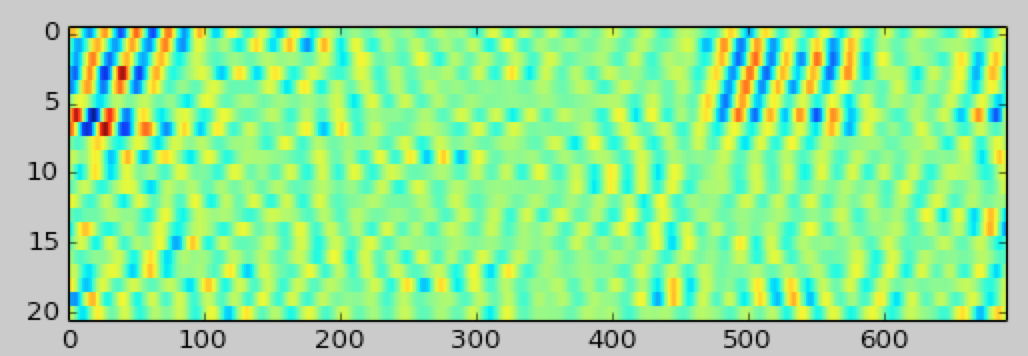
\includegraphics[width=2\columnwidth, height=.8\columnwidth]{plots/x_example.png}
\caption{Input fringe rate filtered frequncy domain data for a single baseline.}
\label{fig:x_example}
\end{figure*}

\begin{figure}[h!]\centering
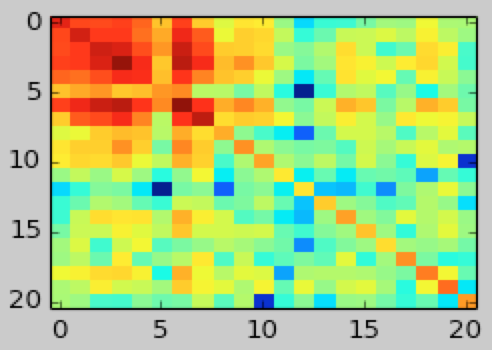
\includegraphics[width=\columnwidth, height=.8\columnwidth]{plots/C_example.png}
\caption{The covariance matix for a single baseline of the frequency data in
figure \ref{fig:x_example}.} 
\label{fig:C_example}
\end{figure}

\begin{figure}[h!]\centering
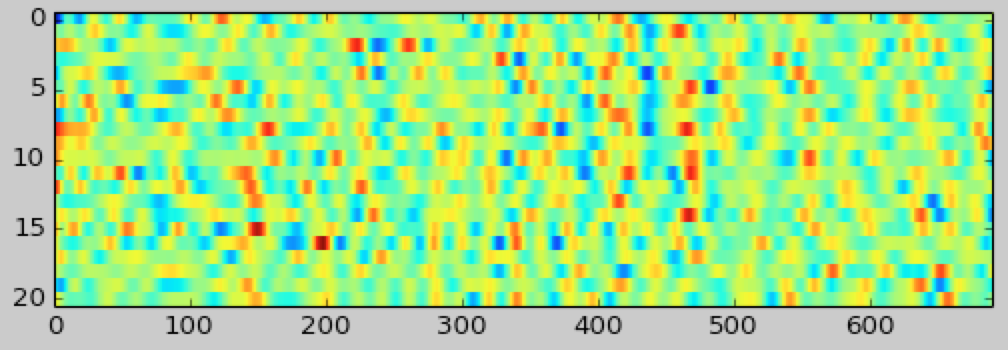
\includegraphics[width=\columnwidth, height=.8\columnwidth]{plots/_Cx_example.png}
\caption{Frequency vs. time data of a single baseline weighted by the inverse of
the covariance matrix shown in figure \ref{fig:C_example}} 
\label{fig:_Cx_example}
\end{figure}

\begin{figure}[h!]\centering
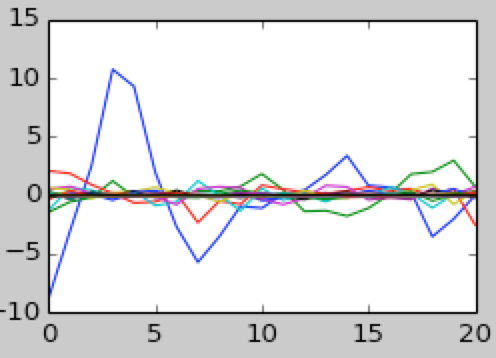
\includegraphics[width=\columnwidth, height=.8\columnwidth]{plots/lamV_example.png}
\caption{The eigeinmodes of the covariance matrix in figure \ref{fig:C_example}
weighted by their corresponding eigeinvalue.} 
\label{fig:lamV_example}
\end{figure}

\begin{figure}[h!]\centering
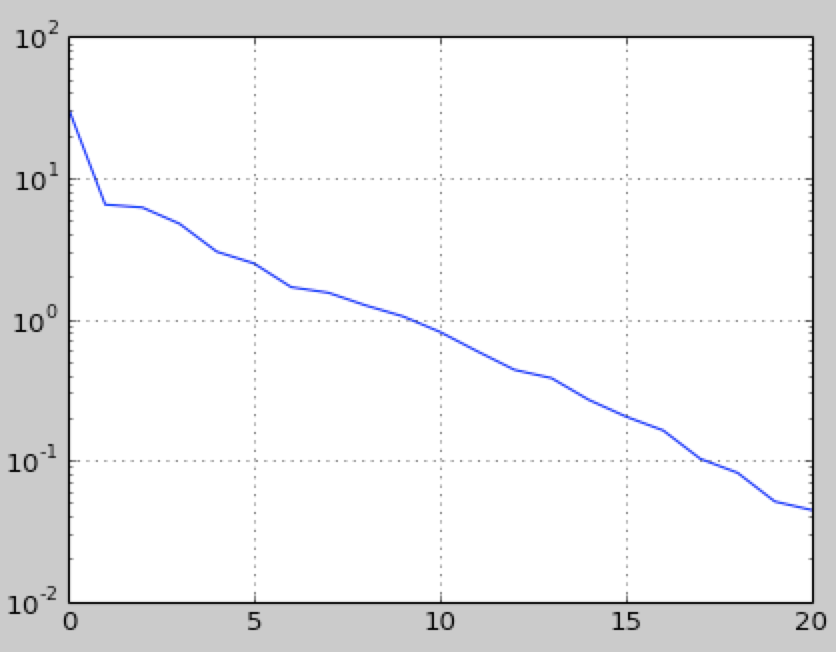
\includegraphics[width=\columnwidth, height=.8\columnwidth]{plots/lam_example.png}
\caption{The eigen spectrum of the covaraince matrix for a singel baseline.}
\label{fig:lam_example}
\end{figure}


\section{Summary of Improvements from PSA32}
XXX Should this section be here XXX
In comparison to the previous PAPER pipeline (see \cite{parsons_et_al2014a}),
this analysis took a slightly different approach which included some critical
steps to improve our upper limit. In short, the improvements included using a
new, refined redundant calibration method (Zheng 2014), increasing the width of
the wideband delay filter that removes smooth spectrum foregrounds, weighting
the lst binned data sets, and optimal fringe rate filtering. In section
\ref{sec:analysis}, we dicuss each of the improvements in more detail.

Figure \ref{fig:step_through_pspec} (TBD) shows the power spectra when each of
the steps mentioned above are turned off and for the one where all of them are
turned on. We can see the gradual improvement of the power spectra (hopefully).



%A more rigorous calibrations. Forward Ref.
%omnical
%lstbinning with chi-sq weighting
%horizon cut at 200ns = 100 + 100 (instead of 100 + 15)
%optimal fringe-rate filtereing
%want the 4(5?) figures in this section. Incrementally step back through improvement points.



\section{Results}
%   -Tsys, and Tsys vs. time ?
\subsection{Noise Levels}

%
%   -Final Pspecs and from various stages 
%       --before/after omnical: Data in
%           /data2/home/zakiali/psa_live/forlstbinning for the before data set.
%           Currently being binned.
%           Note that this data set has ~271 fewer files ~ 48 hours. Hence, it
%           is not the same as the omnical data set.
%           After data set is the one we have always been using : 
%           /data2/home/zakiali/psa_live/forlstbinning_omnical_2 :
%           lstbin_even and lstbin_odd.
%       --before/after frf. Ditto in the above directories.
%       --before after foregrounds. There is foreground data in there as well.
%       SHould we make a foreground run with the non omnical set as well.
\subsection{Power Spectrum}
Figure \ref{fig:final_pspec} shows the speherically averaged power spectrum we
measure. 
Figure \ref{fig:final_posterior} shows the posterior distribution of the power
spectrum by fitting a flat (in $\Delta^{2}$) curve to the powerspectrum
assuming gaussian error bars.
%
%   -Implications for polarized foregrounds.
%       --Flip this around on David and James : We don't see anything at this
%         level, which implies such and such for polarized emission.
%   -Radio recombination and other unsmooth foregrounds. 
%       --paper by peng, Oh. We could maybe confirm this??
%   -Summarize Jonnie's Result.
%   -Repeat the science measurement in Parsons 2014. This will compliment the
%    Jonnies result.
%   -the wedge - maybe?
\begin{figure*}[h!]\centering
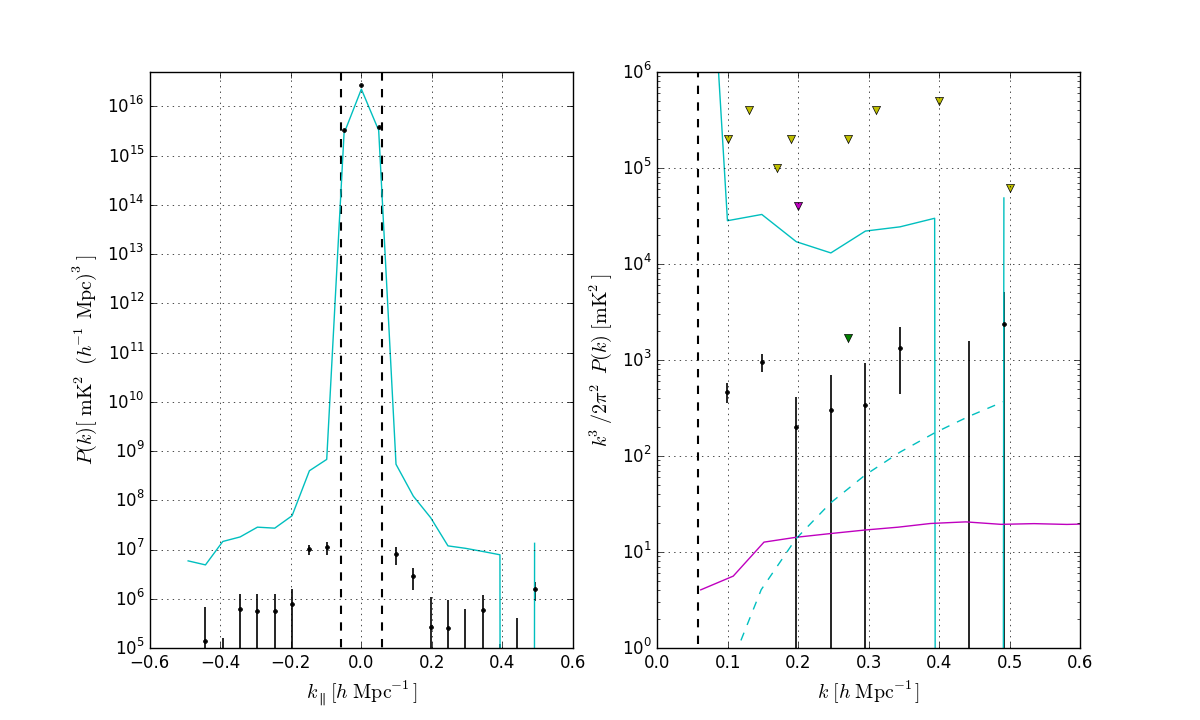
\includegraphics[width=1.5\columnwidth, height=1\columnwidth]{plots/pk_k3pk.png}
\caption{The final power spectrum result.}
\label{fig:final_pspec}
\end{figure*}

\begin{figure}[h!]\centering
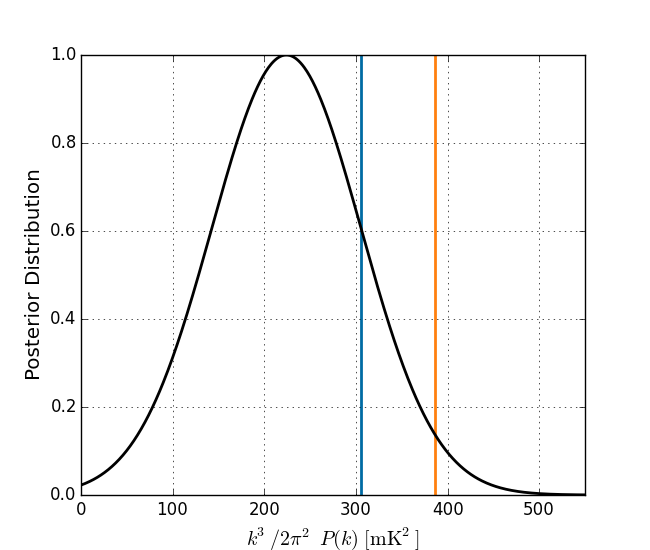
\includegraphics[width=\columnwidth, height=.8\columnwidth]{plots/flat_k3pk_posterior.png}
\caption{The posteriror distributiom assuming a flat, gaussian spectrum in $\Delta^{2}$.}
\label{fig:final_posterioir}
\end{figure}


\section{Discussion}
%   -Future datasets. Things to look forward to.
%
%   -HERA
%
%   -Relative merrits of foreground avoidance vs fg filtering.
%
%   -relative importance of improvements of psa32.
%
%   -vamp on consistency with zero.
%
%   -Remaining challenges.
%
%       --Polarization leakage.
%       --Sensitivity 
%       --Seeing foregrounds.
%
%
%
%
\section{Conclusions}


%\clearpage
%\nocite{*}
\bibliographystyle{apj}
\bibliography{biblio}

\end{document}

